%%====================================================
%% Literatuurstudie
%%====================================================

\chapter{Literatuurstudie}
\label{ch:literatuurstudie}

Het maken van ERP-software is een exclusieve wereld waar toetreden als een nieuwkomer niet vanzelfsprekend is. Toch is het merkwaardig dat SAP, de leider in deze markt, de 3e grootste softwareleverancier is ter wereld. Enkele alternatieven zijn: NetSuite, Microsoft Dynamics of bv. een eigen implementatie.
De grootste vraag die we ons stellen is hoe het requirements management proces bij een ERP-implementatie verloopt, welke impact dit heeft op het resultaat en gerelateerde activiteiten die je moet uitvoeren als je een implementatie in de praktijk moet uitvoeren. 

Het requirements management proces is een 1e stap richting een succesvol project \autocite{Williamson2018}, op deze manier heeft de organisatie een overzicht over de gewenste functionaliteiten en prioriteiten. De populairste manier om deze schema's te maken is met BPMN maar er zijn alternatieven beschikbaar zoals: Storytelling, Flow-oriented Process models... \autocite{Lillehagen2009}. De verzameling van deze documenten wordt doorgaans als RICE (Reports, Interfaces, Conversions en Extensions) \autocite{Williamson2018} en zorgt er voor dat elk aspect van het project verwerkt is zodat de organisatie klaar is voor de transitie van de huidige operaties. 

De 2 varianten van pakketten die wij bekijken zijn off-the-shelf software en maatwerk met parametrisatie waarbij maatwerk een off-the-shelf implementatie neemt en deze op verschillende manieren gaat customizen om het naar de vrager zijn hand te zetten \autocite{Vollmer2016}. Vaak is het een moeilijke beslissing, custom software lijkt op het 1e zicht goedkoper en waarom zou je als ontvanger geen systeem willen dat volledig is aangepast aan jouw bedrijf. Er moet namelijk rekening gehouden worden met de 'verborgen' kosten die verbonden zijn aan het customizen, het is noodzakelijk dat deze systemen up to date blijven maar een aangepast systeem is meestal complexer (en dus duurder) om bij te werken \autocite{Bdc2019}. Vaak is de business afhankelijk van dit systeem. De gedachte dat het bedrijf waarvan je ondersteuning krijgt er plots mee stopt is iets dat ondernemers 's nachts wakker houdt. Een groot voordeel van een SAP implementatie is dat het systeem makkelijk overdraagbaar is aan een ander bedrijf. Hoe meer parameters, hoe langer het zal duren vooraleer je nieuwe leverancier zicht ingewerkt heeft. Bij een volledig nieuw systeem zonder gemeenschappelijke basis zal praktisch elke leverancier je aanraden om over te schakelen. Deze beslissing heeft een impact op de kost en leveringsduur van het systeem, het is logisch dat je een langere opleveringstermijn hebt bij een implementatie met veel parameters.

Agile werken weegt zwaar op het samenwerken, organisatie en het afleveren van veranderingen waardoor er geen hoop informatie beschikbaar moest zijn om een project te starten zoals bij de watervalmethode \autocite{Mrpeasy2018}. De stappen om een ERP-systeem agile te implementeren zijn als volgt. De beginfase bestaat uit het opmaken van de product backlog waarop je alle technische requirements gaat verzamelen, dit al dan niet gegeven door de klant of via een ander bedrijf. Deze stap wordt algemeen gezien als 'Telling the story'. Veel bedrijven doen dit in de vorm van user story mapping, afbeelding \ref{fig:mapping} is hier een voorbeeld van. Hierna gaat het bedrijf aan de slag met hun off the shelf product dat beschikbaar is, worden ze worden ook wel Independent Software Vendors genoemd \autocite{Mrpeasy2018} . Het is dus de bedoeling dat men verschillende modules gaat selecteren en eventueel aanpassingen voorzien zodat die overeen komen met de requirements die op de backlog staan. De sprint wordt dan gebruikt om functionaliteiten beschikbaar te maken (bv. data entry strategy ontwikkelen) en deze verder te personaliseren. Het grote verschil met de agile methodiek zoals wij die kennen is dat bepaalde taken in 1 grote blok staan en deze niet opgesplitst kunnen worden omdat ze gewoonweg niet zullen werken als je maar een deel van de module ontwikkelt. Bij elke sprint is er dan weer opvolging van de klant die dan het project in de huidige toestand kan evalueren en bijsturen. Het grote voordeel is dat de implementatie zeer flexibel is terwijl je er toch op kan rekenen dat het systeem bepaalde bedrijfsprocessen zal ondersteunen.

\begin{figure}[b!]
    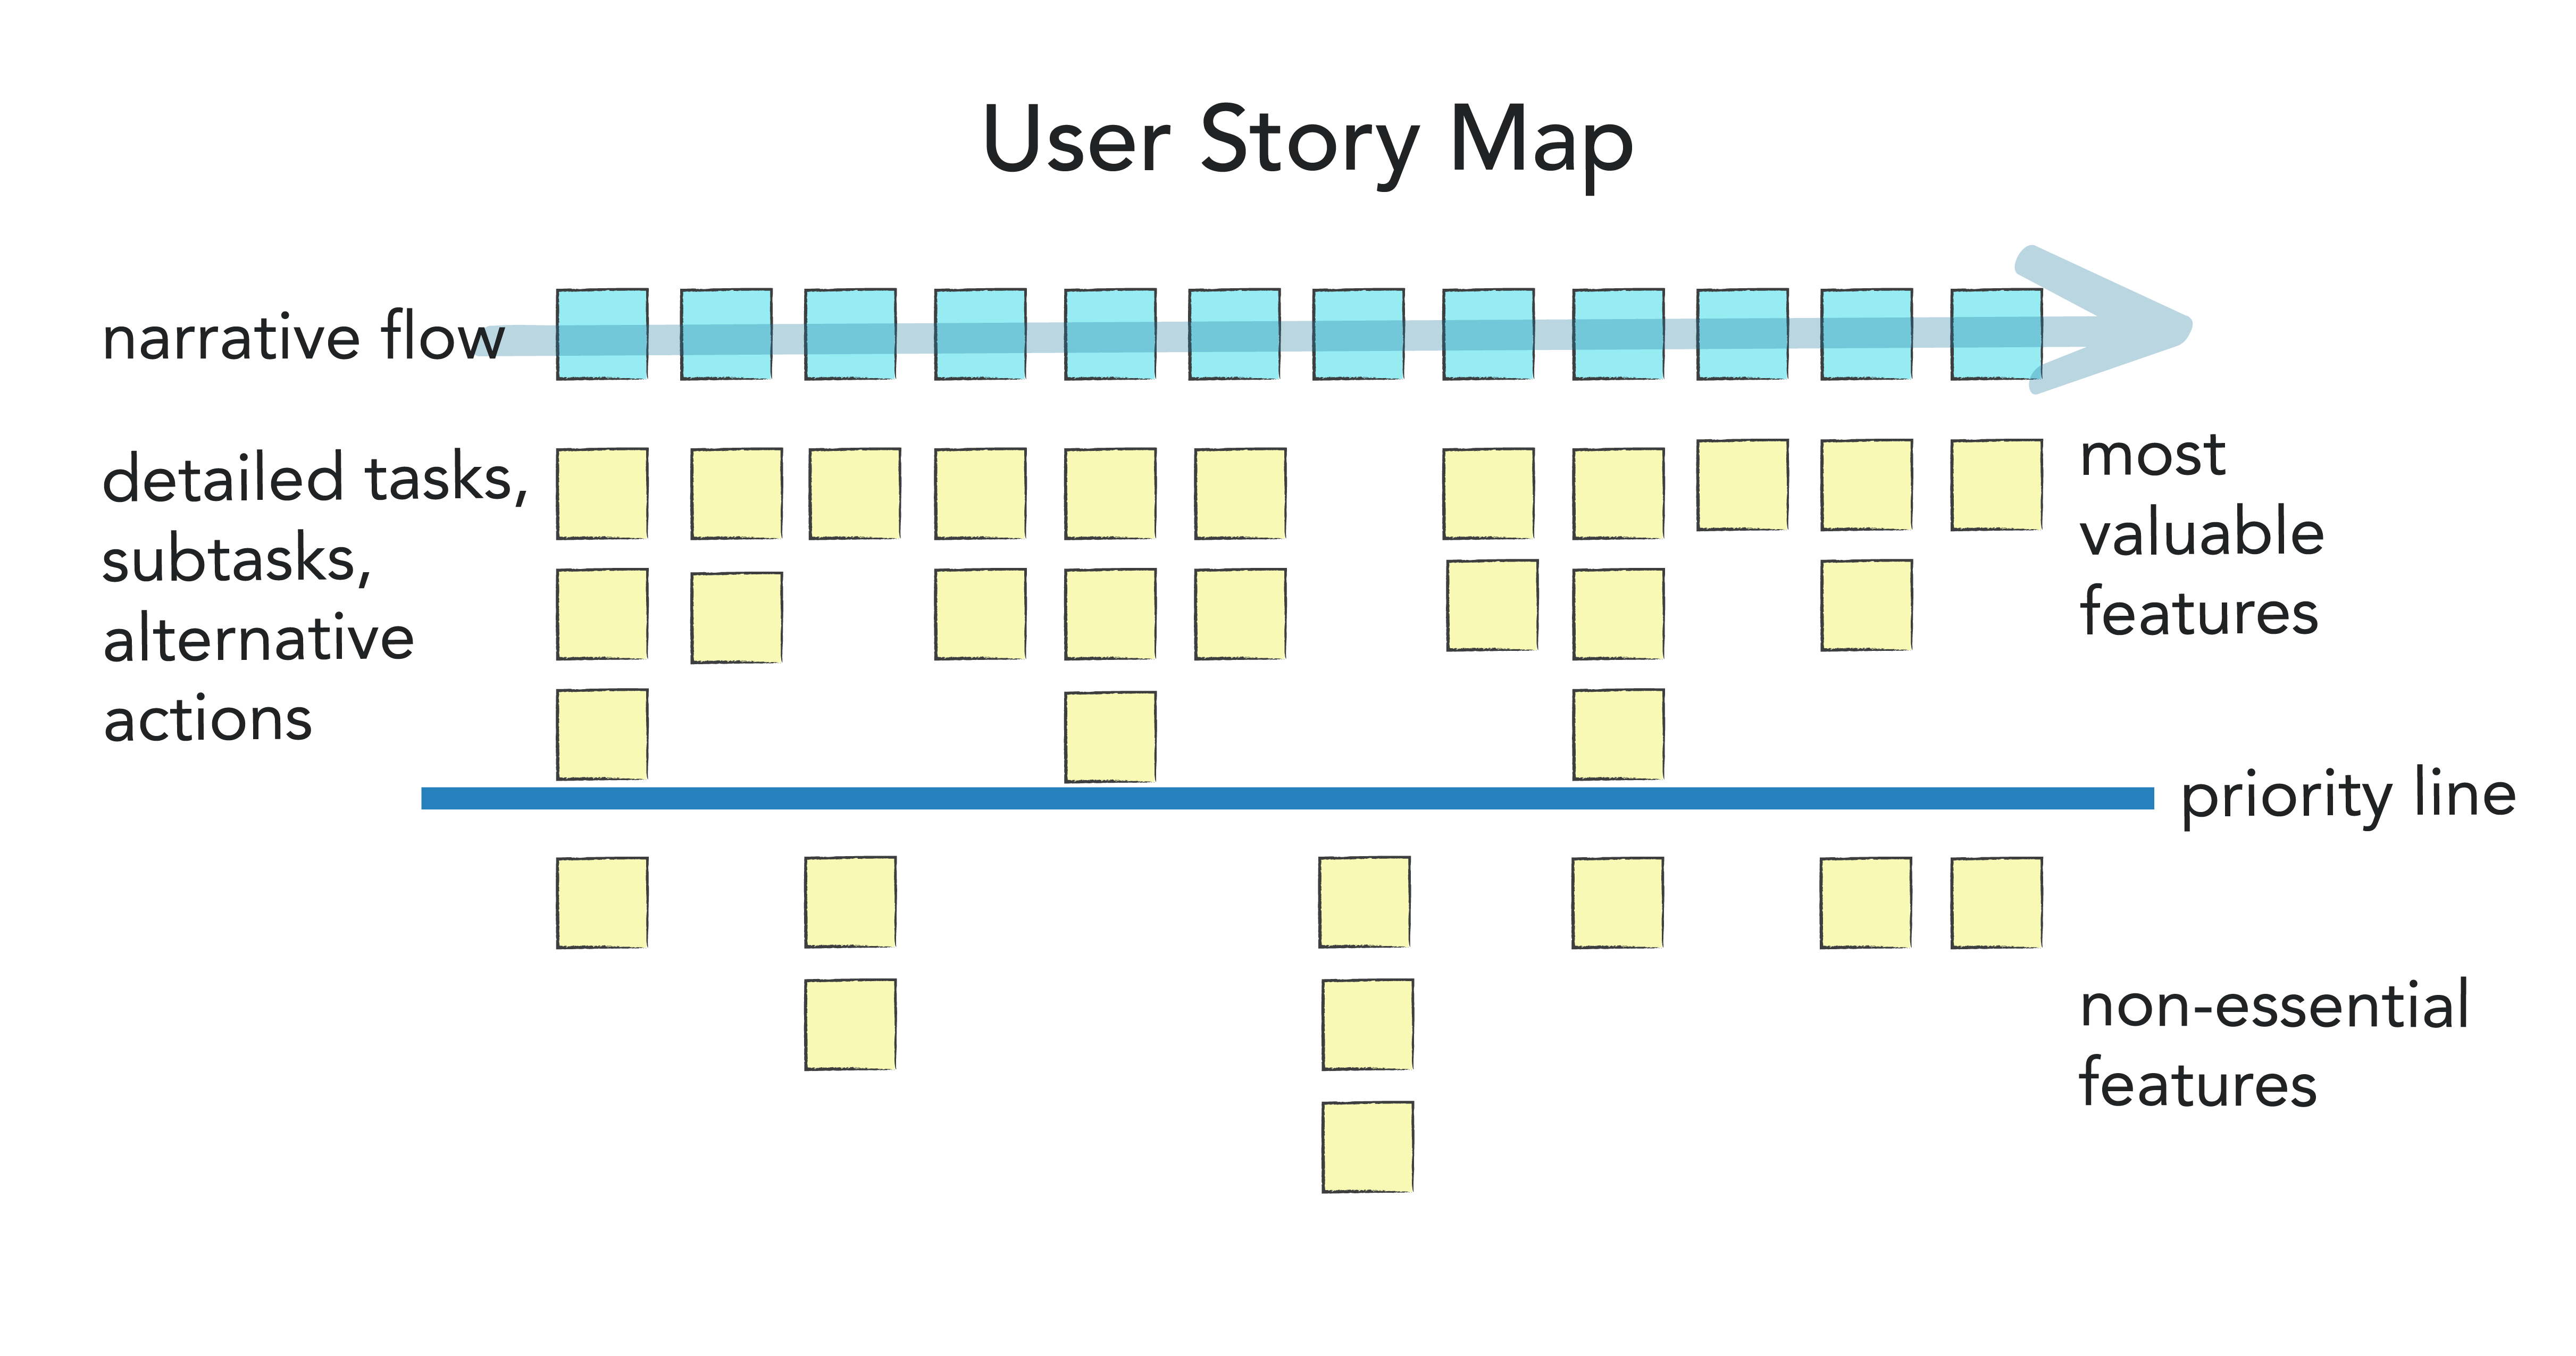
\includegraphics[width=\linewidth]{mapping.png}
    \caption{User story mapping}
    \label{fig:mapping}
\end{figure}